%!TEX root = ../Main.tex
\section{Fabrication of Copper Test Filter}

Once the design was finalised we plotted the circuit in Protel and had photo masks made. We also made masks to verify our method of calculating resonator coupling coefficients. Fabrication consisted of spinning photo resist onto the Duroid board, exposing it with the mask under UV light then etching. The copper filter is shown in Figure \ref{figure:test-copper-open}, and resonator boards are shown in Figure \ref{figure:test-resonator-open}.

\begin{figure}[ht]
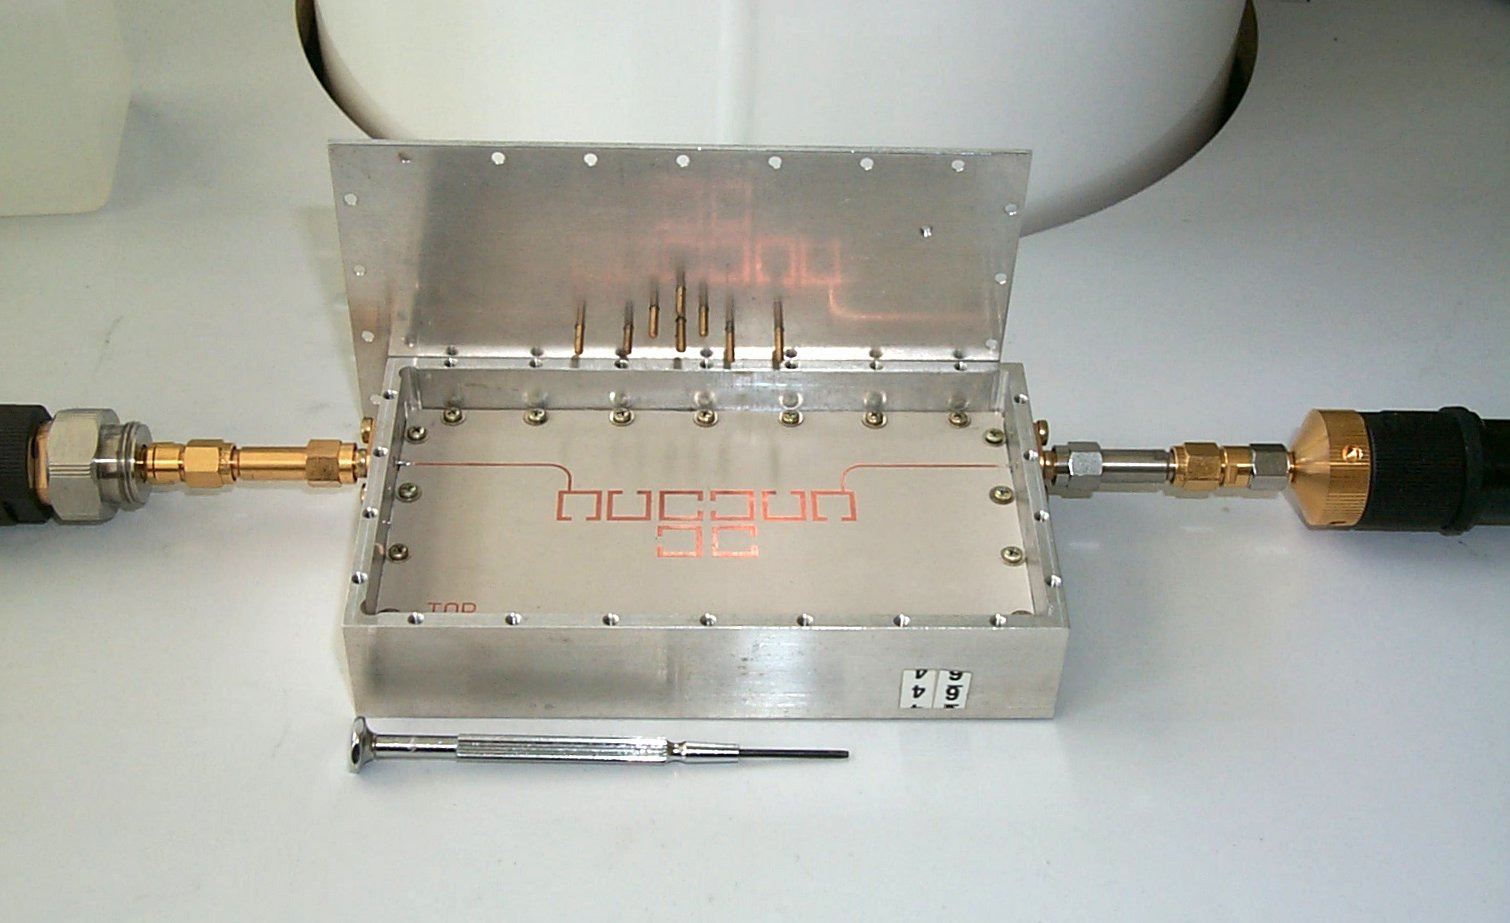
\includegraphics[scale=0.25]{fig/test-copper-open.jpg}
\vspace{-1em}
\caption{Copper test filter}
\label{figure:test-copper-open}
\end{figure}

\begin{figure}[ht]
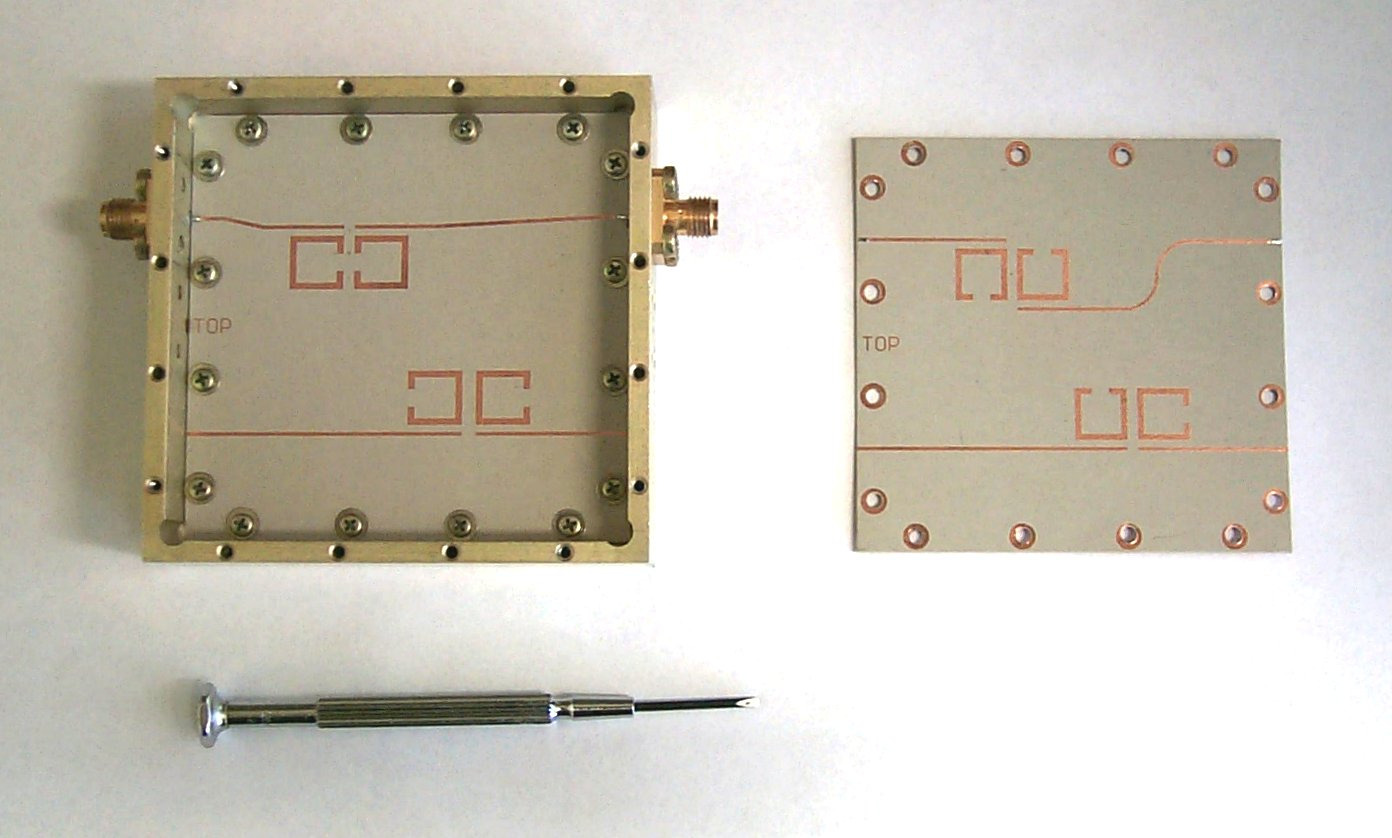
\includegraphics[scale=0.25]{fig/test-resonator-open.jpg}
\vspace{-1em}
\caption{Boards to test resonator coefficients}
\label{figure:test-resonator-open}
\end{figure}


% ------------------------------------------------------------------
\subsection{Testing}
Once tuned, the filter was measured to have the response shown in Figure 14. The lid appeared to reduce the stray couplings between non-adjacent resonators and improve the filter response. This effect was also observed when the HTS filter was tested.

\begin{figure}[ht]
\hspace{-4em}
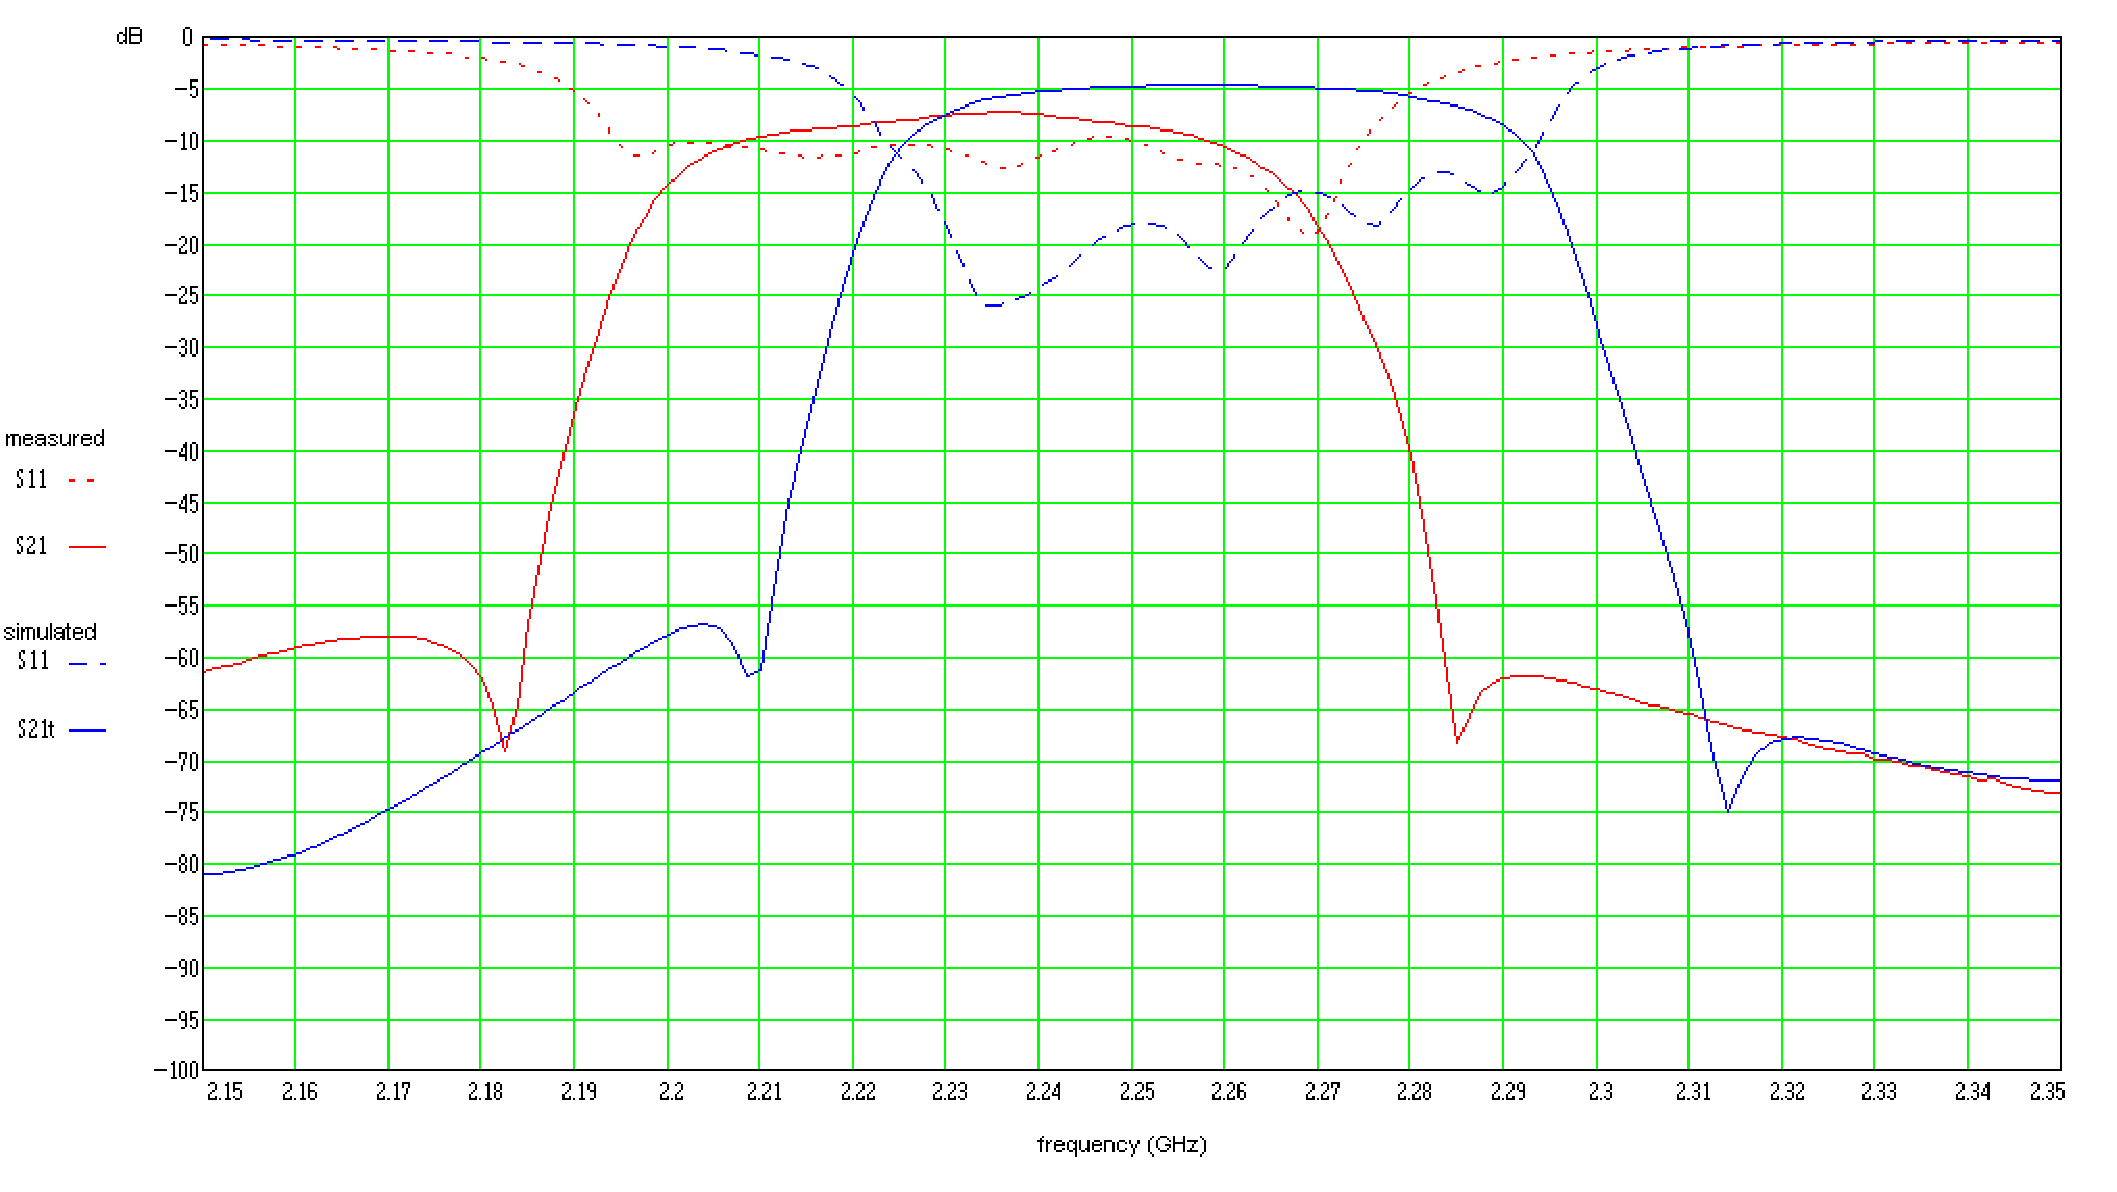
\includegraphics[scale=0.4]{fig/test-copper-response.pdf}
\vspace{-1em}
\caption{Response of copper test filter}
\label{figure:test-copper-response}
\end{figure}

\begin{figure}[ht]
\hspace{-4em}
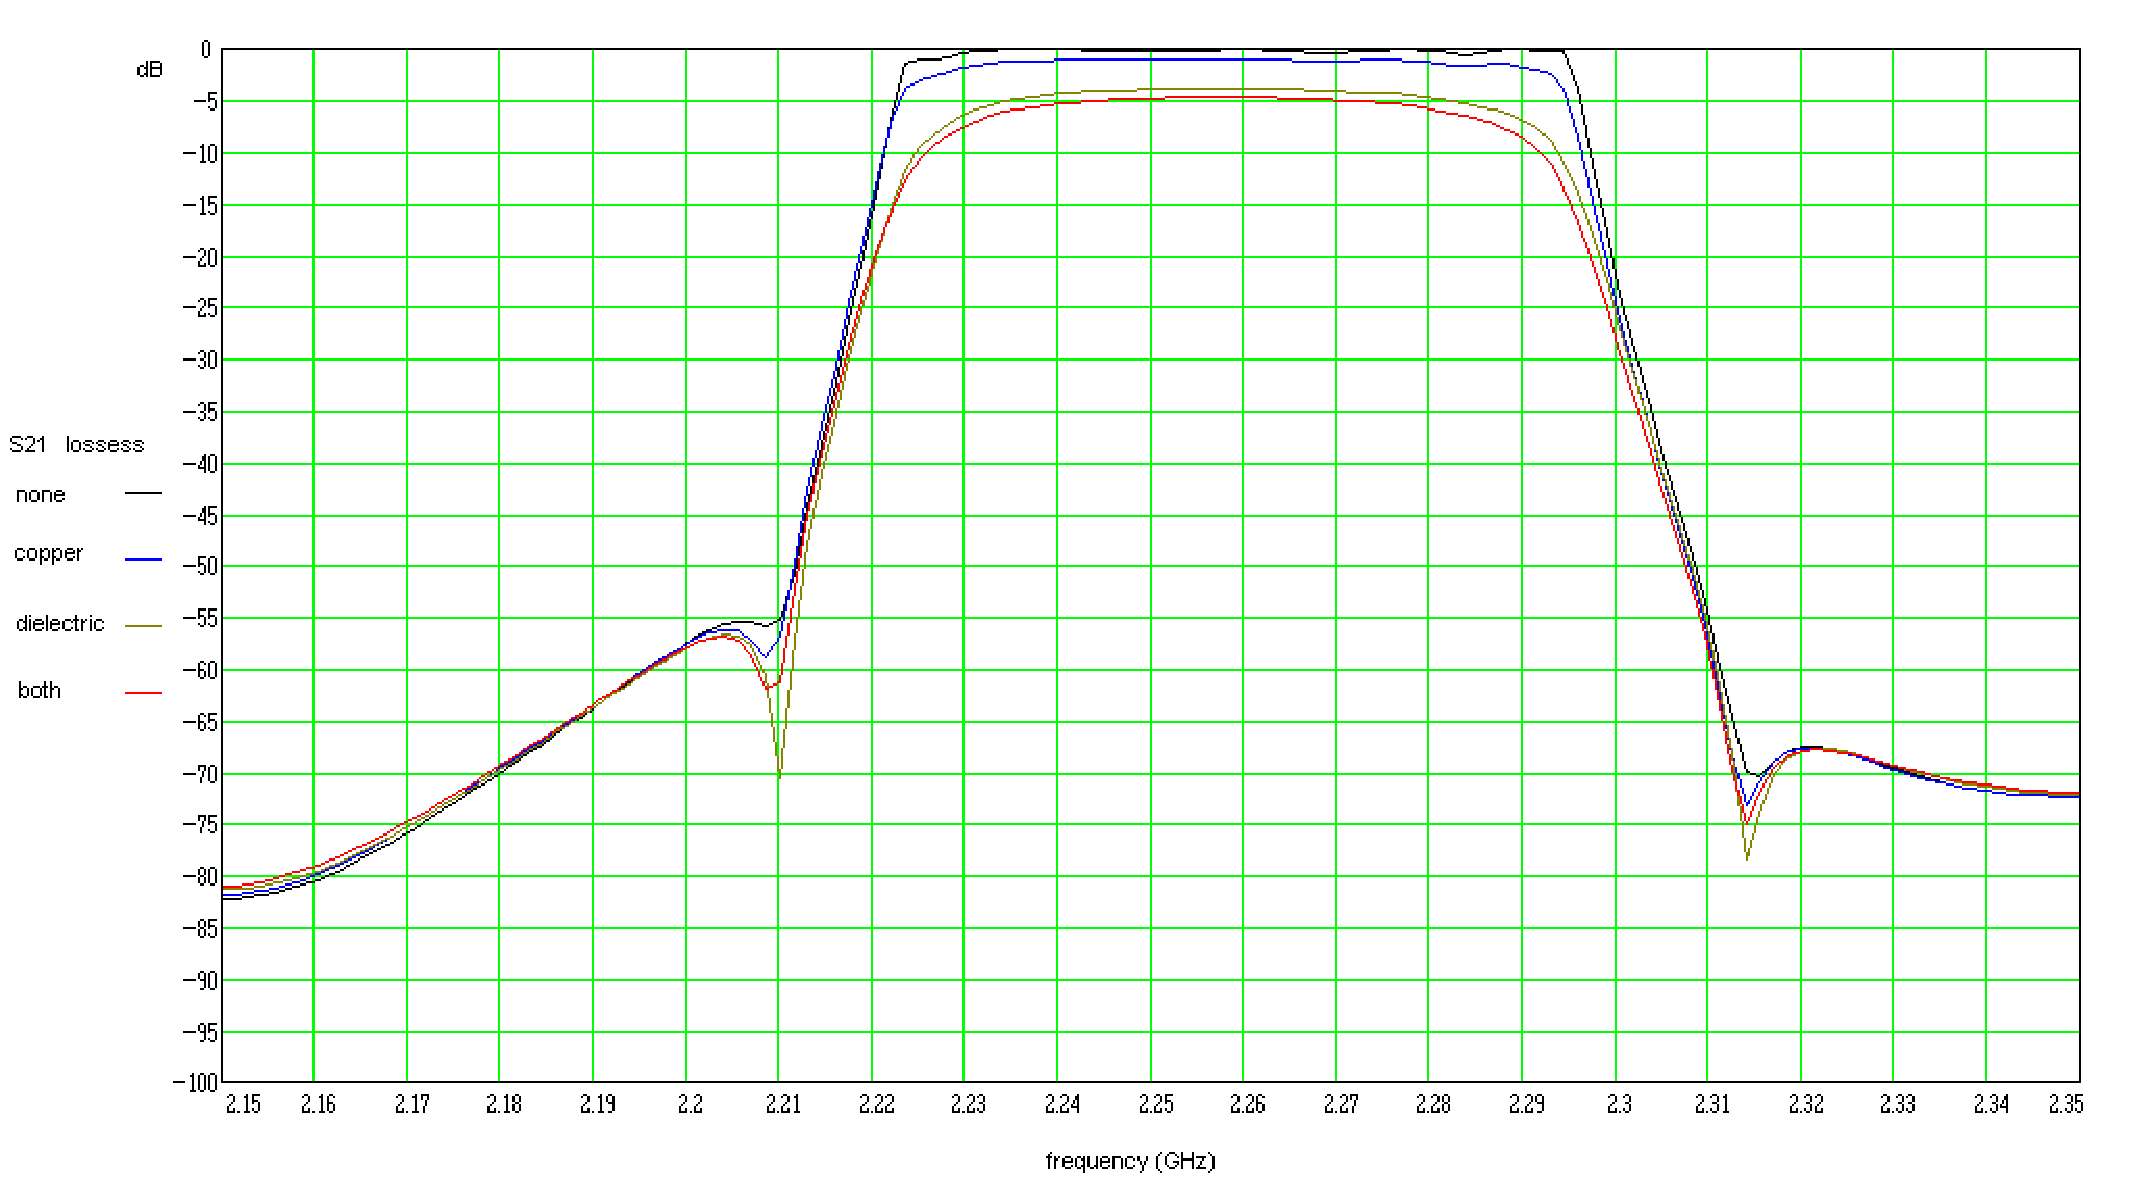
\includegraphics[scale=0.4]{fig/test-copper-loss.pdf}
\vspace{-1em}
\caption{Loss mechanisms}
\label{figure:test-copper-loss}
\end{figure}

The filter center frequency was about 25MHz too low and examination under the microscope revealed that it had been slightly over etched and had lost about 0.03mm all the way around. We simulated the filter with revised dimensions but it did not create the same effect. This leads us to believe that either the dielectric constant or height of the material is slightly different than what was specified. 

The rounding of the filter passband is due to copper and dielectric losses which we verified with the simulator (see figure 15). Examination of the diagram reveals that although there is a loss from the finite conductivity of copper, the large proportion is due to the loss tangent of the substrate (RT/Duroid 6010.5 loss tangent = 0.0023).

After seeing this we checked the loss tangent of the substrate material which we were planning to use for the HTS filter, Lanthanum Aluminate, LaAlO3. We was happy to discover that its loss tangent of 6.0E-5 compared with 2.3E-3 would present no problem.

With a filter of such a small fractional bandwidth (3 percent) we had expected to do a bit of tuning. Our next step was to obtain a lid and plant a forest of tuning screws which could be screwed down into the gap between the resonators. Each screw slightly decreased the fringe field in the gap and served to reduce the coupling between two resonators. This allowed us to slightly alter the stop band response. The lid with the screws can be seen in Figure 12.

To correct the center frequency of the filter we experimented with the possibility of trimming a few hundred microns off the end of the resonators with a razor knife. The characterisation boards came in useful for this purpose as their were 8 resonators which we could butcher and directly see the effect on frequency and coupling. 

With a steady hand it was possible to trim lengths of line equivalent to approximately 5MHz at a time off the ends of the resonators. The effect on the coupling coefficients depends on the types of coupling the resonator being modified is a part of. Electric coupling is most effected as the majority of the action takes place via electric fringe fields at the ends of the resonators. Conversely, magnetic coupling is least effected as the magnetic fringe fields circulates the lengths of the resonators away from the ends.

From simulation it was determined that even trimming of the lines does not significantly effect the shape of the filter response as it is shifted by a few tens of MHz. However, reproducibility between hand modifications is difficult to obtain. With more practice and frequent examinations under a measuring microscope it should be possible to trim down the resonators and center the filter on the correct frequency though this has not yet been attempted.

Apart from fabrication tolerances, this prototype was deemed a success and gave a degree of confidence to the HTS design.
